\section{Das Modell}
Im folgenden Abschnitt soll das in \ref{fig:ccmodel} gezeigte Modell zur Beschreibung von DNS-Cloud-Services detailliert erläutert werden. Dies soll zum Verständnis und als Hilfe bei der Anwendung dienen. Außerdem soll es die gewählte Darstellungsform und Notation beleuchten, die zur Erstellung des Modells genutzt wurde.

\begin{sidewaysfigure*}[]
    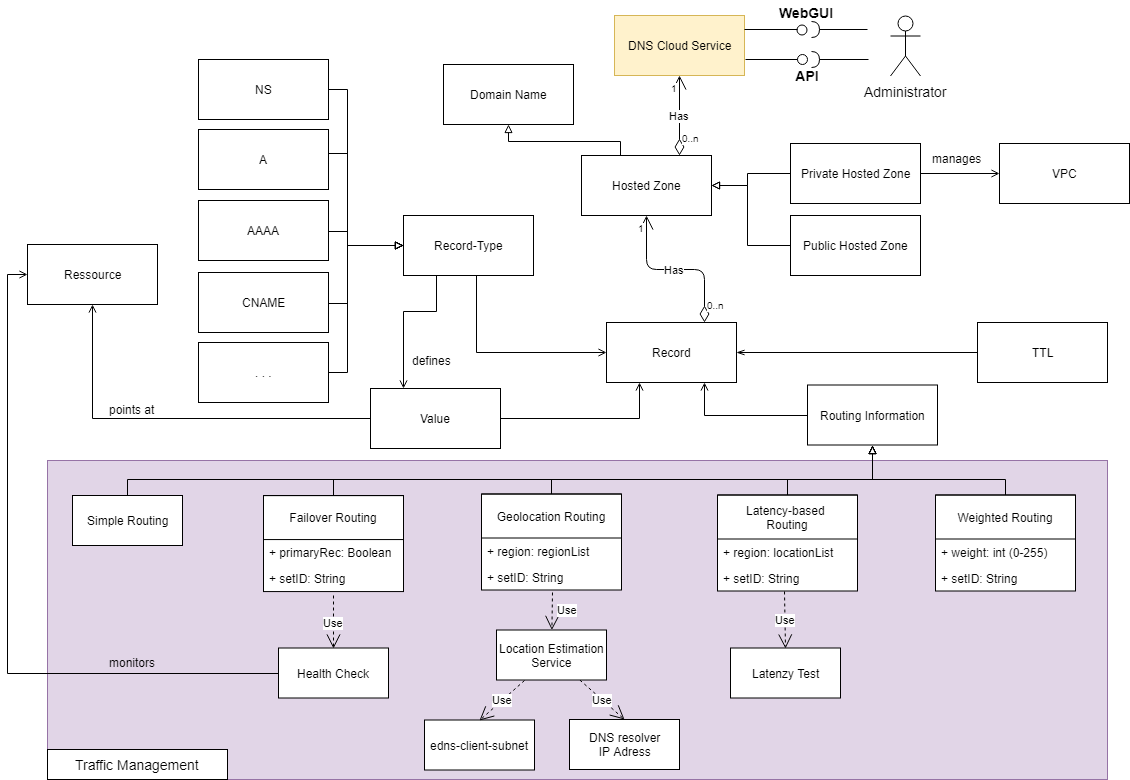
\includegraphics[width=\textwidth]{images/cc_modelxml.png}
    \caption{Modell zur Beschreibung von DNS-Cloud-Services}
    \label{fig:ccmodel}
\end{sidewaysfigure*}

\subsection{Schnittstellen}
Zur Nutzung der DNS-Cloud-Services allgemein stehen unterschiedliche Möglichkeiten zur Verfügung. Wird ein neues Benutzerkonto angelegt, geschieht dies über eine Weboberfläche. Nach der Einrichtung ist es möglich über die Benutzeroberfläche der Internetseite auf das Produktportfolio des Dienstleisters zuzugreifen. Sämtliche Interaktionen mit dem Cloud-Service sind über diese Weboberfläche möglich. So kann der Kunde jederzeit und von jedem internetfähigen Gerät, plattformunabhängig über den Browser seines Betriebssystems auf die Services zugreifen. Das bedeutet, dass keine Installation von zusätzlichen Anwendungen oder Treibern notwendig ist.

Eine weitere Möglichkeit ist der Zugriff über eine Schnittstelle zur Anwendungsprogrammierung (API). Diese Schnittstellen ermöglichen es mit der Hilfe von Kommandozeilenwerkzeugen auf die Services des Cloud-Providers zuzugreifen. Somit können auch ohne die Hilfe des Webinterfaces administrative Aufgaben bezüglich der Cloud erledigt werden. Eine API ermöglicht es ebenfalls über Skriptsprachen Routineaufgaben zu automatisieren oder den Cloud-Service in eine unternehmensinterne Software einzubinden. Dies bringt den Vorteil eines flexibleren Umgangs und einer bessere Einbindung des Cloud-Services in die alltäglichen Prozesse.

 \subsection{Hosted Zones}
Bei der Analyse der einzelnen DNS-Cloud-Dienstleistungen fällt auf, dass das zentrale Element die sogenannten Hosted-Zones darstellen. Sie dienen als Container zum Hosten der DNS-Einträge zu einer bestimmten Domäne und umschließen somit alle Informationen über die Weiterleitung des Datenverkehrs dieser.
Ein DNS-Cloud-Service kann über mehrere Hosted-Zones verfügen. Die Namensgebung findet hierbei meist über den Domain-Namen statt. Somit wird die Funktion der Hosted-Zones schnell ersichtlich. Außerdem ist über den Domain-Namen eine einzigartige Identifizierung der unterschiedlichen Zonen gewährleistet. Je nach DNS-Cloud-Dienstleistung kann jedoch auch ein abweichender Name zur betreffenden Domain gewählt werden. Laut den offiziellen Dokumenationen der Cloud-Provider, liegt das Limit an Hosted-Zones standardmäßig bei über 100 Hosted-Zones, bei allen drei untersuchten Anbietern.

\subsection{Private und Public Hosted-Zones}
Hosted-Zones können in zwei unterschiedliche Kathegorien aufgeteilt werden. Diese Kathegorien beschreiben die Art des Netzwerkes, die durch die Zone verwaltet werden soll. \textit{Public-Hosted-Zones} enthalten DNS-Einträge, welche die Weiterleitung für öffentlich zugängliche Domänen beschreiben. Sie sind also zuständig für die Weiterleitung im Internet und es ist somit notwendig die dort erforderlichen Konventionen für DNS-Einträge zu erfüllen.
\textit{Private-Hosted-Zones} stellen Container dar, die Informationen zur Verwaltung der Kommunikation eines privaten Netzwerkes zu Verfügung stellen. Sie ermöglichen die Weiterleitung innerhalb einer \textit{Virtual Private Cloud (VPC)} oder auch VPC übergreifend über unterschiedliche Services des Cloud-Providers. Dies bedeutet, dass der DNS-Service vom Internet abgekoppelt ist und somit auch Domain-Namen verwendet werden können, an denen man selbst keine offiziellen Rechte besitzt. Bei der Erstellung einer solchen Private-Hosted-Zone muss ein vorhandenes VPC angegeben werden, dem diese folgend zugeordnet werden kann.

\subsection{Domain-Name}
Wie zuvor erwähnt basieren Hosted-Zones auf einem zugehörigen Domain-Namen. Befindet man sich in einer Private-Hosted-Zone kann dieser frei gewählt werden. Soll die Domain jedoch über das Internet erreichbar sein, ist zunächst eine Registrierung des Domain-Name über einen externen Dienstleister erforderlich. Sollte der Cloud-Dienstleister keine Möglichkeit zu Verfügung stellen einen Domain-Namen zu registrieren, ist eine Weiterleitung von dem Domain-Name-Provider auf den DNS-Cloud-Dienst einzurichten. Dies ist meistens über das Onlineportasl des jeweiligen Dienstleisters möglich.

\subsection{Records}
Wie zuvor beschrieben, enthalten Hosted-Zones DNS-Einträge, die Informationen zur Weiterleitung bezüglich einer bestimmten Domain kapseln. Diese Einträge werden in unserem als Records bezeichnet. Jeder Record besteht aus einem Record-Typen, einem Value einem TTL-Wert und je nach Provider eventuellen Routing Informationen. Ein Record erhält außerdem noch einen Namen einer Domain oder Subdomain und endet immer mit dem Namen der Hosted-Zone.

\subsection{Value}
Wird ein Record aufgerufen, liefert dieser einen zugewiesenen Wert zurück. Dieser Wert wird im Modell als Value bezeichnet. Der Value eines Records ist somit die enthaltene Hauptinformation. Der eingetragene Wert wird durch den Record-Type bestimmt.


\subsection{Record-Types}
Record-Types definieren sowohl die Art des Records, als auch die Inhalte, die dieser enthält.
Im Modell wurde nur eine Auswahl an Record-Types aufgeführt. Die übrigen Typen werden durch das Objekt mit den drei Punkten dargestellt. Folgend sollen die Record-Types, welche in allen drei untersuchten DNS-Cloud-Services vorzufinden sind kurz mit den von ihnen erwarteten Werten vorgestellt werden.

\subsubsection{A}
wird genutzt um einer Domäne eine IPv4-Adresse zuzuweisen. Der Value ist eine IPv4-Adresse.

\subsubsection{AAAA}
wird verwendet um einer Domäne eine IPv6-Adresse zuzuweisen. Der Value ist eine IPv6-Adresse.

\subsubsection{CNAME}
ist die Kurzform für \textit{Canonical Name}. Wird verwendet um Alias-Datensätze zu erstellen. Das Value-Format ist das gleiche wie der Recordname.

\subsubsection{MX}
gibt an unter welchem Domain-Name ein Mail-Server zur bezeichneten Domain zu Verfügung steht. Hier können mehrere Mail-Server eingetragen werden, deswegen gibt es einen zweiten Wert der die Priorität angibt. Die Priorität wird in ganzzahligen numerischen Werten beschrieben. Mail-Server mit der niedrigeren Prioritäten-Zahl werden bevorzugt genutzt. Der Value setzt sich somit aus einem ganzzahligen Wert und einer A- oder AAAA-Adresse zusammen.

\subsubsection{NS}
ist ein essenzieller Eintrag für die Hosted-Zone. Der NS-Record identifiziert die für die Hosted-Zone zu verwendenden autoritativen DNS-Server. Er wird bei der Erstellung einer Hosted-Zone automatisch angelegt und es werden außerdem bei allen untersuchten Providern vier verschiedene Nameserver zugewiesen.

\subsubsection{SRV}
wird verwendet um IP-basierte Dienste in einer Domain zu propagieren. Der Value besteht aus vier verschiedenen Werten, die durch Leerzeichen voneinander abgetrennt werden. Die ersten drei einzutragenden Werte bestehen aus Dezimalzahlen und repräsentieren die Priorität, Gewichtung den den zu zuständigen Port. Anschließend wird ein Domain-Name angehängt.

\subsubsection{TXT}
wird verwendet um der angegebenen Domain einen oder mehrere Zeichenfolgen zuzuweisen. Jede dieser Zeichenfolgen kann bis zu 255 Zeichen beinhalten. Bei mehreren Zeichenfolgen werden diese von den Clients verkettet und anschließen wie eine einzelne lange Zeichenfolge behandelt. Innerhalb der Zeichenketten können neben alphanumerischen Zeichen auch Leerzeichen und ausgewählte Sonderzeichen verwendet werden.

\subsubsection{PTR}
wird meist für Reverse-Lookup verwendet. Ist quasi das Gegenstück zum A- oder AAAA-Record-Type. Sie dienen dazu einen Domain-Name für eine bestimmte IP-Adresse zu identifizieren.

\subsection{TTL}
Hier kann der Time-to-Live Wert für den DNS-Record angegeben werden. Dieser gibt an, wie lange der DNS-Record bei rekursiven DNS-Servern im Cache als gültig angesehen werden darf. Als Maßeinheit werden Sekunden genutzt. 

Die Argumente, die für eine kürzere oder längere TTL sprechen wurden bereits in Abschnitt \ref{lab:ttl} diskutiert. Außerdem wurde eine Best-Practice Methode aufgezeigt, die bei bevorstehenden Änderungen am System eingesetzt werden kann um einen reibungslosen Übergang zwischen Änderungen zu gewährleisten. Hinzuzufügen ist, dass Amazon aws Route53 als Empfehlung gibt einen Wert von cirka 60 Sekunden anzugeben, falls ihr Health-Check Service in Anspruch genommen wird.
